\section{Why learn scales}

Learning scales may sound boring. And, if you learn it without context, it indeed may be boring. However, scales are the foundation of music.

When a house doesn't have a good foundation, it can easily be destroyed by natural phenomena. But having a good foundation for the main house doesn't stop you from making a beautiful fairy-like garden or a nice painting all over the walls of the house.

The same goes for music. Scales will give you a framework to work with. A set of notes that sound good together. But you can, and should, be creative with how you use this framework. Using notes outside the scale can give some interesting sounds as well when used properly.

Some benefits for example are that you will be able to more easily figure out music by ear and that you will be able to improvise more easily over songs. 

\section{Creating context: playing your first chords}

If you can't wait to play some chords, feel free to have a look at \autoref{fig:guitar_major_minor_chords} right away to learn the basic chord shapes. If you search for songs on the internet with \textit{"<song name> <artist> chords"} you will most likely find a webpage with the chords to play.

Just learning these chord shapes will get you quite far in terms of being able to play along with songs.

But wouldn't it be nice to be able to figure songs out by ear as well, making chords sound more interesting, being able to improvise over a song, and making your own chord progressions? If so, continue with the next sections.

\newpage

\section{Scales and intervals}

A scale is a collection of notes in ascending order between a note and its octave. The two main scales are the major (happy sound) and minor (sad sound) scale.

When describing scales, often the terms "whole" (w) and "half" (h) steps are used. Sometimes you will also see the terms "tone" (T) and "semitone" (S). Moving up a half step on the guitar means moving to the next fret (towards the body). Moving up a whole step is the same as two half steps.

Lets look at the intervals of 1 semitone again (\autoref{tab:guitar_sharp_flat_intervals_chap_5}). Going one step to the left or to the right is a half step interval. To take a whole step, simply take two half steps.

\begin{table}[h]
	\centering
	\begin{tabular}{*{12}{P{5mm}}}
		\large{A} & \large{A\sharp} & \large{B} & \large{C} & \large{C\sharp} & \large{D} & \large{D\sharp} & \large{E} & \large{F} & \large{F\sharp} & \large{G} & \large{G\sharp} \\ \\
		\large{A} & \large{B\flat} & \large{B} & \large{C} & \large{D\flat} & \large{D} & \large{E\flat} & \large{E} & \large{F} & \large{G$\flat$}& \large{G} & \large{A\flat}
	\end{tabular}
	\caption{Sharp and flat intervals. Each step to the left or right is a half step.}
	\label{tab:guitar_sharp_flat_intervals_chap_5}
\end{table}

A list of intervals and their names is shown in \autoref{tab:guitar_intervals_in_octave}. You don't have to learn these by heart as of now. But we will refer to these later on when describing the scales.

\begin{table}[h]
	\centering
	\begin{tabular}{|c|c|c|}
		\hline
		\textbf{Semitones} & \textbf{Name} & \textbf{Symbol} \\
		\hline
		\hline
		0 & Unison & 1 \\
		\hline
		1 & Minor 2nd & 2$\flat$ \\
		\hline
		2 & Major 2nd & 2 \\
		\hline
		3 & Minor 3rd & 3$\flat$ \\
		\hline
		4 & Major 3rd & 3 \\
		\hline
		5 & Perfect 4th& 4 \\
		\hline
		6 & Augmented 4th / Diminished 5th / Tritone & 4$\sharp$ / 5$\flat$ \\
		\hline
		7 & Perfect 5th & 5 \\
		\hline
		8 & Minor 6th & 6$\flat$ \\
		\hline
		9 & Major 6th / Diminished 7th & 6 / 7$\flatflat$ \\
		\hline
		10 & Minor 7th & 7$\flat$ \\
		\hline
		11 & Major 7th & 7 \\
		\hline
		12 & 8th (octave)& 8 \\
		\hline
	\end{tabular}
	\caption{Intervals in an octave}
	\label{tab:guitar_intervals_in_octave}
\end{table}

\newpage

\subsection{The major scale}

As mentioned. The most common scales are the major and minor scales. A lot of music theory is based on the major diatonic scale. A diatonic scale means that it has 7 different notes in the scale where each letter only occurs once. So the major diatonic scale is the first one we will learn.

Each scale has a formula. For the major diatonic scale the formula is shown in (\autoref{tab:guitar_major_scale_interval}). On the top you see the steps between each note (the formula itself). The numbers indicate the interval of the note in the scale. Note 1 and 8 are the same note. But the 8 is one octave higher than the 1.

\begin{table}[h]
	\centering
	\begin{tabular}{*{16}{c}}
		& \multicolumn{2}{P{4mm}}{\large{W}} & \multicolumn{2}{P{4mm}}{\large{W}} & \multicolumn{2}{P{4mm}}{\large{H}} & \multicolumn{2}{P{4mm}}{\large{W}} & \multicolumn{2}{P{4mm}}{\large{W}} & \multicolumn{2}{P{4mm}}{\large{W}} & \multicolumn{2}{P{4mm}}{\large{H}} & \\
		\multicolumn{2}{P{4mm}}{1} & \multicolumn{2}{P{4mm}}{2} & \multicolumn{2}{P{4mm}}{3} & \multicolumn{2}{P{4mm}}{4} & \multicolumn{2}{P{4mm}}{5} & \multicolumn{2}{P{4mm}}{6} & \multicolumn{2}{P{4mm}}{7} & \multicolumn{2}{P{4mm}}{8}
	\end{tabular}
	\caption{Major scale intervals}
	\label{tab:guitar_major_scale_interval}
\end{table}

Note that \autoref{tab:guitar_sharp_flat_intervals_chap_5} has 12 different notes/pitches. Now count the total amount of half steps that are shown in \autoref{tab:guitar_major_scale_interval} (a whole step is two half steps). Indeed, there are 12 half steps to go from the note at note 1 to the same note one octave higher (note 8).

For example, to create the C major scale we will start on the C and then simply follow the formula.

\begin{table}[h]
	\centering
	\begin{tabular}{*{16}{c}}
		& \multicolumn{2}{P{4mm}}{\large{W}} & \multicolumn{2}{P{4mm}}{\large{W}} & \multicolumn{2}{P{4mm}}{\large{H}} & \multicolumn{2}{P{4mm}}{\large{W}} & \multicolumn{2}{P{4mm}}{\large{W}} & \multicolumn{2}{P{4mm}}{\large{W}} & \multicolumn{2}{P{4mm}}{\large{H}} & \\
		\multicolumn{2}{P{4mm}}{1} & \multicolumn{2}{P{4mm}}{2} & \multicolumn{2}{P{4mm}}{3} & \multicolumn{2}{P{4mm}}{4} & \multicolumn{2}{P{4mm}}{5} & \multicolumn{2}{P{4mm}}{6} & \multicolumn{2}{P{4mm}}{7} & \multicolumn{2}{P{4mm}}{8} \\
		\multicolumn{2}{P{4mm}}{C} & \multicolumn{2}{P{4mm}}{D} & \multicolumn{2}{P{4mm}}{E} & \multicolumn{2}{P{4mm}}{F} & \multicolumn{2}{P{4mm}}{G} & \multicolumn{2}{P{4mm}}{A} & \multicolumn{2}{P{4mm}}{B} & \multicolumn{2}{P{4mm}}{C}
	\end{tabular}
	\caption{C major scale}
	\label{tab:guitar_c_major_scale}
\end{table}

\iffalse
The G major scale is shown below in (\autoref{tab:guitar_g_major_scale}).

\begin{table}[h]
	\centering
	\begin{tabular}{*{16}{c}}
		& \multicolumn{2}{P{4mm}}{\large{W}} & \multicolumn{2}{P{4mm}}{\large{W}} & \multicolumn{2}{P{4mm}}{\large{H}} & \multicolumn{2}{P{4mm}}{\large{W}} & \multicolumn{2}{P{4mm}}{\large{W}} & \multicolumn{2}{P{4mm}}{\large{W}} & \multicolumn{2}{P{4mm}}{\large{H}} & \\
		\multicolumn{2}{P{4mm}}{1} & \multicolumn{2}{P{4mm}}{2} & \multicolumn{2}{P{4mm}}{3} & \multicolumn{2}{P{4mm}}{4} & \multicolumn{2}{P{4mm}}{5} & \multicolumn{2}{P{4mm}}{6} & \multicolumn{2}{P{4mm}}{7} & \multicolumn{2}{P{4mm}}{8} \\
		\multicolumn{2}{P{4mm}}{G} & \multicolumn{2}{P{4mm}}{A} & \multicolumn{2}{P{4mm}}{B} & \multicolumn{2}{P{4mm}}{C} & \multicolumn{2}{P{4mm}}{D} & \multicolumn{2}{P{4mm}}{E} & \multicolumn{2}{P{4mm}}{F\sharp} & \multicolumn{2}{P{4mm}}{G}
	\end{tabular}
	\caption{G major scale}
	\label{tab:guitar_g_major_scale}
\end{table}
\fi

In \autoref{tab:guitar_natural_note_major_scale} you see the major scales of all the natural notes. You don't need to remember these by heart at the moment. You do need to learn the formula of the major scale by heart. There are three things to note:

\begin{enumerate}
	\item \textbf{Each scale only has unique letters}. Therefore the 4th note in the F major scale is a B$\flat$ and not an A$\sharp$.
	\item The 5th note in the scale is the start of the scale on the next row. Of course, this is because they are listed as such now. But it is the basis of the "circle of fifths" which we will learn more about later.
	\item Each scale below another in this list has one more $\sharp$ than the previous. And the notes that have a sharp in one scale, also have a sharp in the scales below it. Again, this has to do with the "circle of fifths".
\end{enumerate}

\begin{table}[h]
	\centering
	\begin{tabular}{*{16}{c}}
		& \multicolumn{2}{P{4mm}}{\large{W}} & \multicolumn{2}{P{4mm}}{\large{W}} & \multicolumn{2}{P{4mm}}{\large{H}} & \multicolumn{2}{P{4mm}}{\large{W}} & \multicolumn{2}{P{4mm}}{\large{W}} & \multicolumn{2}{P{4mm}}{\large{W}} & \multicolumn{2}{P{4mm}}{\large{H}} & \\
		\multicolumn{2}{P{4mm}}{1} & \multicolumn{2}{P{4mm}}{2} & \multicolumn{2}{P{4mm}}{3} & \multicolumn{2}{P{4mm}}{4} & \multicolumn{2}{P{4mm}}{5} & \multicolumn{2}{P{4mm}}{6} & \multicolumn{2}{P{4mm}}{7} & \multicolumn{2}{P{4mm}}{8} \\
		\multicolumn{2}{P{4mm}}{F} & \multicolumn{2}{P{4mm}}{G} & \multicolumn{2}{P{4mm}}{A} & \multicolumn{2}{P{4mm}}{B\flat} & \multicolumn{2}{P{4mm}}{C} & \multicolumn{2}{P{4mm}}{D} & \multicolumn{2}{P{4mm}}{E} & \multicolumn{2}{P{4mm}}{F} \\
		\multicolumn{2}{P{4mm}}{C} & \multicolumn{2}{P{4mm}}{D} & \multicolumn{2}{P{4mm}}{E} & \multicolumn{2}{P{4mm}}{F} & \multicolumn{2}{P{4mm}}{G} & \multicolumn{2}{P{4mm}}{A} & \multicolumn{2}{P{4mm}}{B} & \multicolumn{2}{P{4mm}}{C} \\
		\multicolumn{2}{P{4mm}}{G} & \multicolumn{2}{P{4mm}}{A} & \multicolumn{2}{P{4mm}}{B} & \multicolumn{2}{P{4mm}}{C} & \multicolumn{2}{P{4mm}}{D} & \multicolumn{2}{P{4mm}}{E} & \multicolumn{2}{P{4mm}}{F\sharp} & \multicolumn{2}{P{4mm}}{G} \\
		\multicolumn{2}{P{4mm}}{D} & \multicolumn{2}{P{4mm}}{E} & \multicolumn{2}{P{4mm}}{F\sharp} & \multicolumn{2}{P{4mm}}{G} & \multicolumn{2}{P{4mm}}{A} & \multicolumn{2}{P{4mm}}{B} & \multicolumn{2}{P{4mm}}{C\sharp} & \multicolumn{2}{P{4mm}}{D} \\
		\multicolumn{2}{P{4mm}}{A} & \multicolumn{2}{P{4mm}}{B} & \multicolumn{2}{P{4mm}}{C\sharp} & \multicolumn{2}{P{4mm}}{D} & \multicolumn{2}{P{4mm}}{E} & \multicolumn{2}{P{4mm}}{F\sharp} & \multicolumn{2}{P{4mm}}{G\sharp} & \multicolumn{2}{P{4mm}}{A} \\
		\multicolumn{2}{P{4mm}}{E} & \multicolumn{2}{P{4mm}}{F\sharp} & \multicolumn{2}{P{4mm}}{G\sharp} & \multicolumn{2}{P{4mm}}{A} & \multicolumn{2}{P{4mm}}{B} & \multicolumn{2}{P{4mm}}{C\sharp} & \multicolumn{2}{P{4mm}}{D\sharp} & \multicolumn{2}{P{4mm}}{E} \\
		\multicolumn{2}{P{4mm}}{B} & \multicolumn{2}{P{4mm}}{C\sharp} & \multicolumn{2}{P{4mm}}{D\sharp} & \multicolumn{2}{P{4mm}}{E} & \multicolumn{2}{P{4mm}}{F\sharp} & \multicolumn{2}{P{4mm}}{G\sharp} & \multicolumn{2}{P{4mm}}{A\sharp} & \multicolumn{2}{P{4mm}}{B}
	\end{tabular}
	\caption{Major scales of all natural notes}
	\label{tab:guitar_natural_note_major_scale}
\end{table}

\newpage

In \autoref{fig:guitar_major_scale_fretboard} different shapes are shown on how the major scale can be played. The numbers correspond to the interval in the scale. These shapes can be moved up and down the fretboard, as long as the distance between the frets stay the same. Shape \autoref{fig:guitar_major_scale_fretboard_single_string} can even be moved up and down the strings. By moving the shape, you will play a different major scale. The scale that you are playing is determined by the root note (the "1" note). In this example we are therefore playing the F$\sharp$ major scale. If you would move all notes up by 1 fret, you would be playing the G major scale.

The different colors in \autoref{fig:guitar_major_scale_fretboard_standard} indicate different octaves. This is the 'standard'/compact major scale shape. Note how the frets with "8/1" indicate the 8 of the previous octave, and the 1 of the next octave.

There are other "shapes" to play the major scale as well, but these shapes don't start on the root (1) note. We will come back to those later.

Learning these shapes by heart makes it easy to improvise over a song. But more important is to see how these shapes relate to the intervals of the major scale. The easiest shape for this is \autoref{fig:guitar_major_scale_fretboard_single_string}. With this shape you can easily recognize the major diatonic scale formula (w-w-h-w-w-w-h). All shapes have the same notes, just played on a different position on the fretboard and possibly in a different octave. The shapes shown below don't cover all possibilities yet.

The F$\sharp$ major scale has the following notes:

\begin{table}[h]
	\centering
	\begin{tabular}{*{16}{c}}
		& \multicolumn{2}{P{4mm}}{\large{W}} & \multicolumn{2}{P{4mm}}{\large{W}} & \multicolumn{2}{P{4mm}}{\large{H}} & \multicolumn{2}{P{4mm}}{\large{W}} & \multicolumn{2}{P{4mm}}{\large{W}} & \multicolumn{2}{P{4mm}}{\large{W}} & \multicolumn{2}{P{4mm}}{\large{H}} & \\
		\multicolumn{2}{P{4mm}}{1} & \multicolumn{2}{P{4mm}}{2} & \multicolumn{2}{P{4mm}}{3} & \multicolumn{2}{P{4mm}}{4} & \multicolumn{2}{P{4mm}}{5} & \multicolumn{2}{P{4mm}}{6} & \multicolumn{2}{P{4mm}}{7} & \multicolumn{2}{P{4mm}}{8} \\
		\multicolumn{2}{P{4mm}}{F$\sharp$} & \multicolumn{2}{P{4mm}}{G$\sharp$} & \multicolumn{2}{P{4mm}}{A$\sharp$} & \multicolumn{2}{P{4mm}}{B} & \multicolumn{2}{P{4mm}}{C$\sharp$} & \multicolumn{2}{P{4mm}}{D$\sharp$} & \multicolumn{2}{P{4mm}}{E$\sharp$} & \multicolumn{2}{P{4mm}}{F$\sharp$}
	\end{tabular}
	\caption{F$\sharp$ major scale}
	\label{tab:guitar_f_sharp_major_scale}
\end{table}

\autoref{tab:guitar_f_sharp_major_scale} demonstrates an important point mentioned earlier. \textbf{A scale only has unique letters}. Note how the 7th scale degree is an E$\sharp$ instead of an F. Generally we wouldn't write E$\sharp$. But because the F$\sharp$ major scale already uses the letter F for F$\sharp$, we can't use F for just F. We have to use E$\sharp$ instead.

\autoref{fig:guitar_f_sharp_major_scale_score_multi_octave} shows the notes that correspond to \autoref{fig:guitar_major_scale_octaves_over_fretboard}.

\begin{figure}[h]
	\centering
	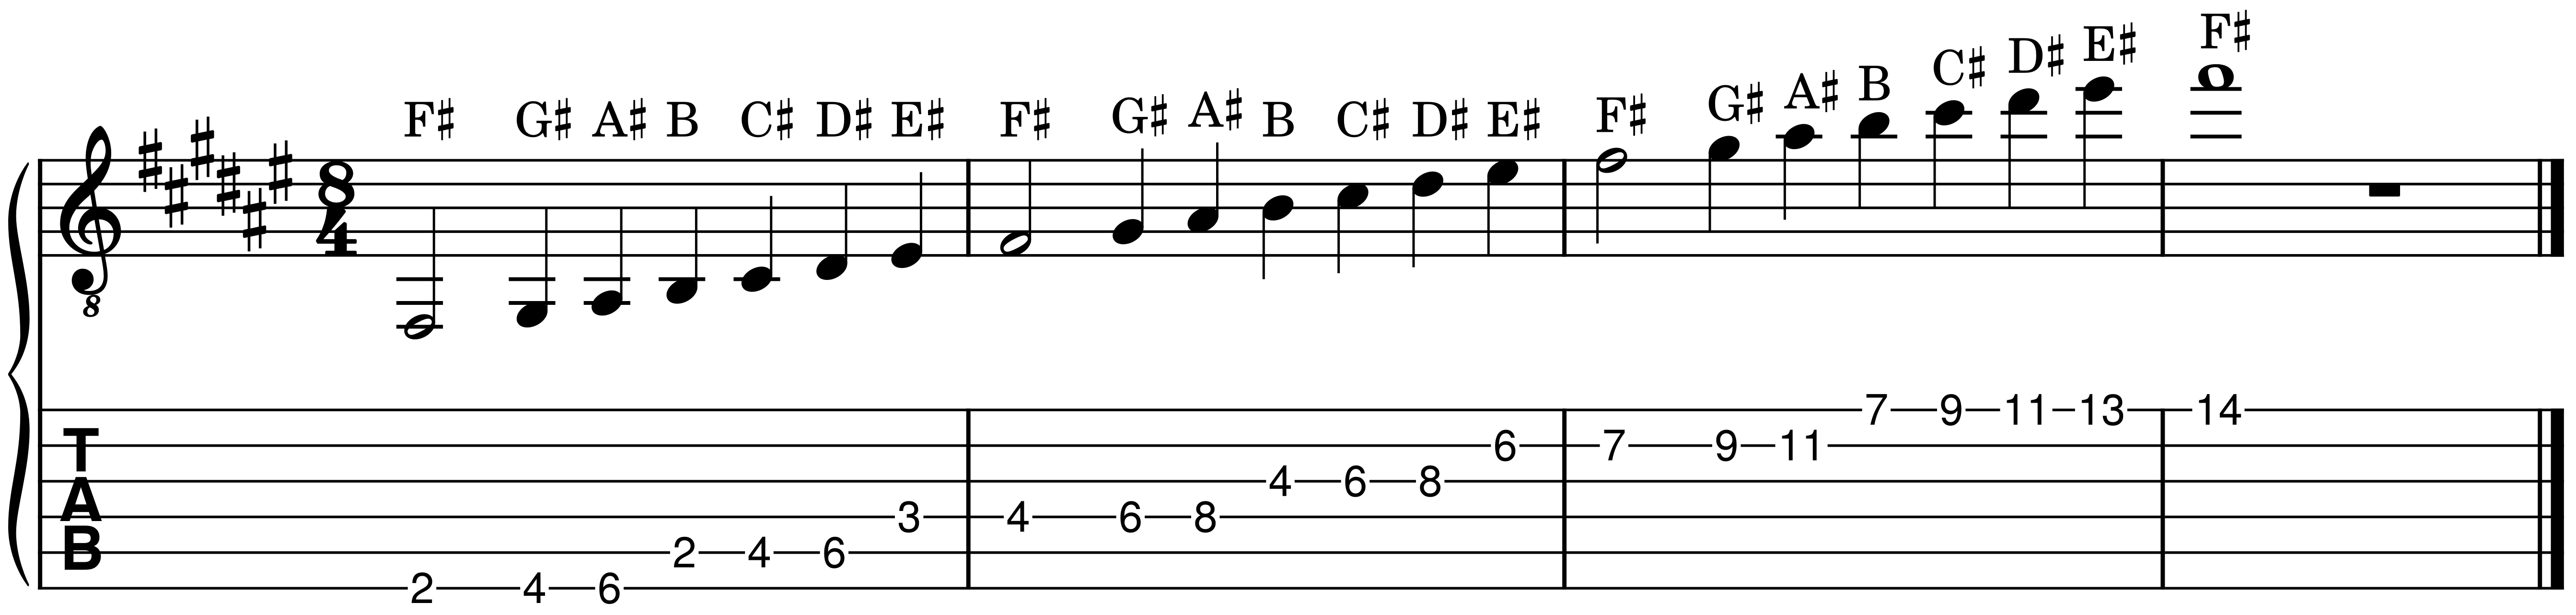
\includegraphics[width=\textwidth]{../../MuseScore/Guitar/GuitarFSharpMajorMultiOctave.png}
	\caption{Multiple octaves of the F$\sharp$ major scale}
	\label{fig:guitar_f_sharp_major_scale_score_multi_octave}
\end{figure}

\newpage

\begin{figure}[h]
	\begin{subfigure}[b]{0.45\textwidth}
		\centering
		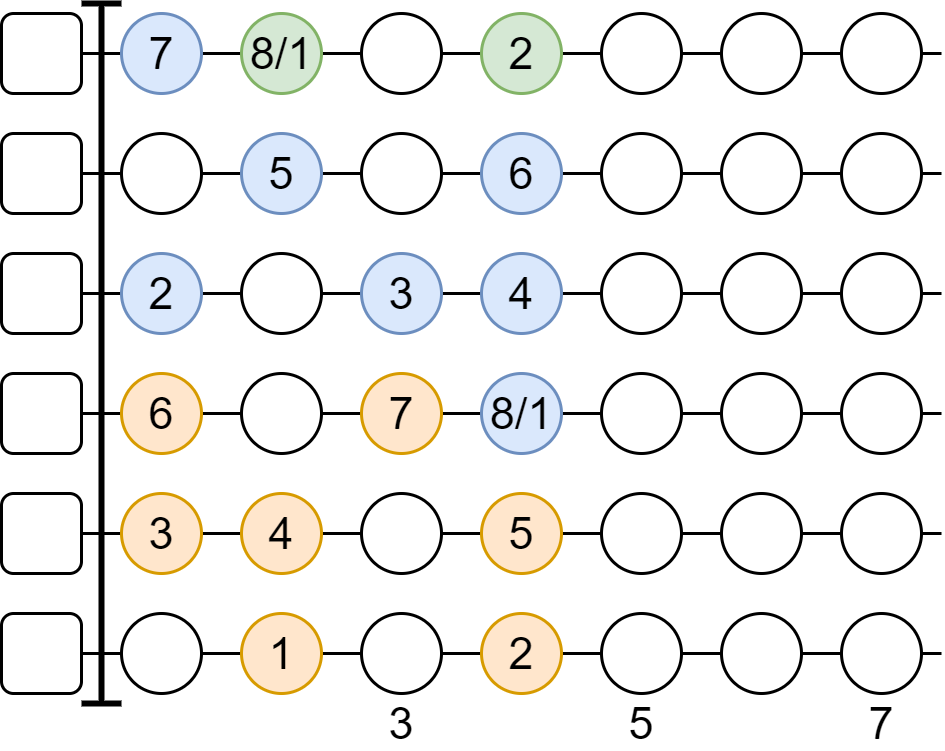
\includegraphics[height=0.18\textheight]{../../Images/guitar_major_scale_standard.png}
		\caption{Major scale on the fretboard (standard)}
		\label{fig:guitar_major_scale_fretboard_standard}
	\end{subfigure}
	\hfill
		
	\vspace{0.5cm}
	\begin{subfigure}[b]{\textwidth}
		\centering
		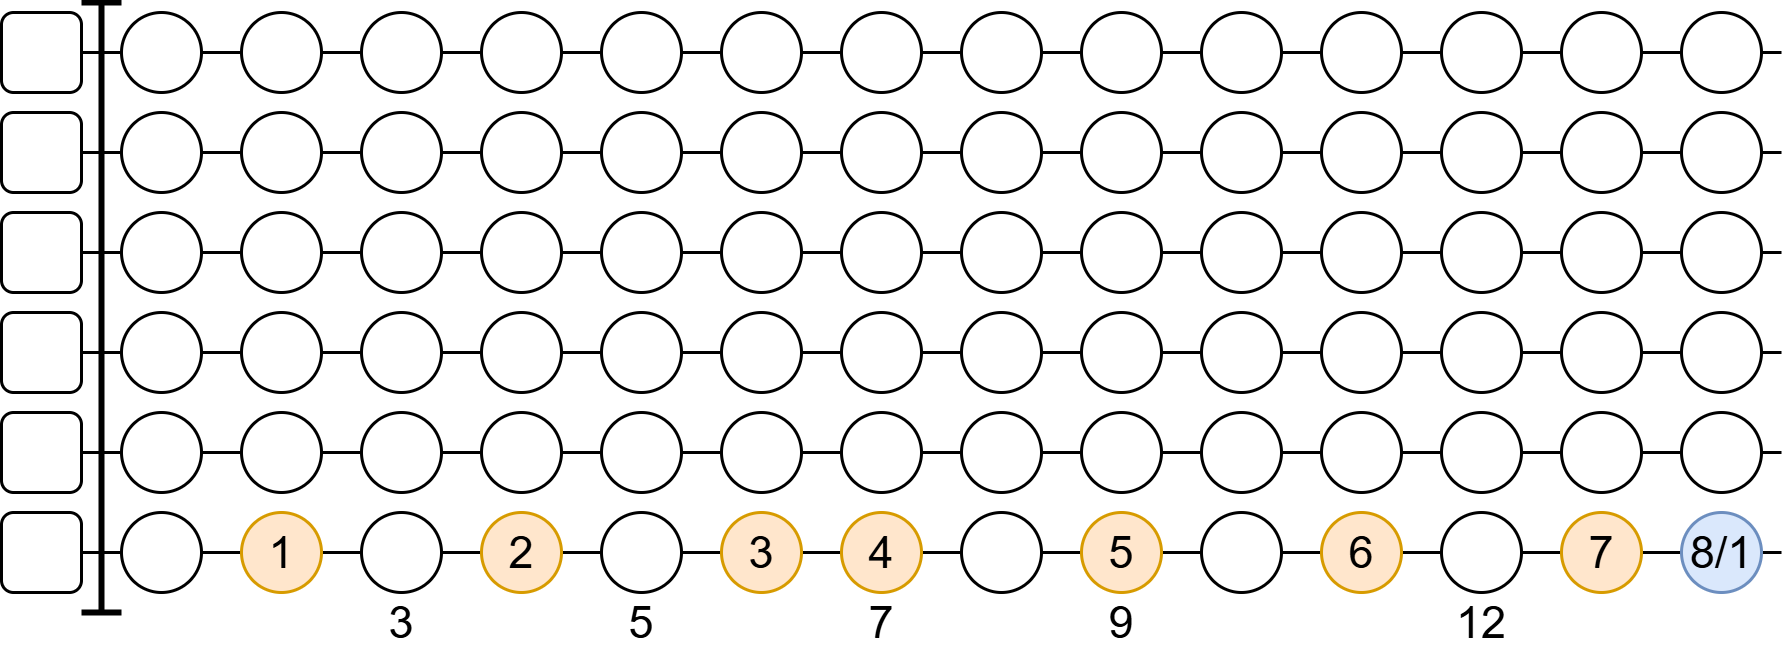
\includegraphics[height=0.18\textheight]{../../Images/guitar_major_scale_single_string.png}
		\caption{Major scale on the fretboard on a single string}
		\label{fig:guitar_major_scale_fretboard_single_string}
	\end{subfigure}
	
	\vspace{0.5cm}
	\begin{subfigure}[b]{\textwidth}
		\centering
		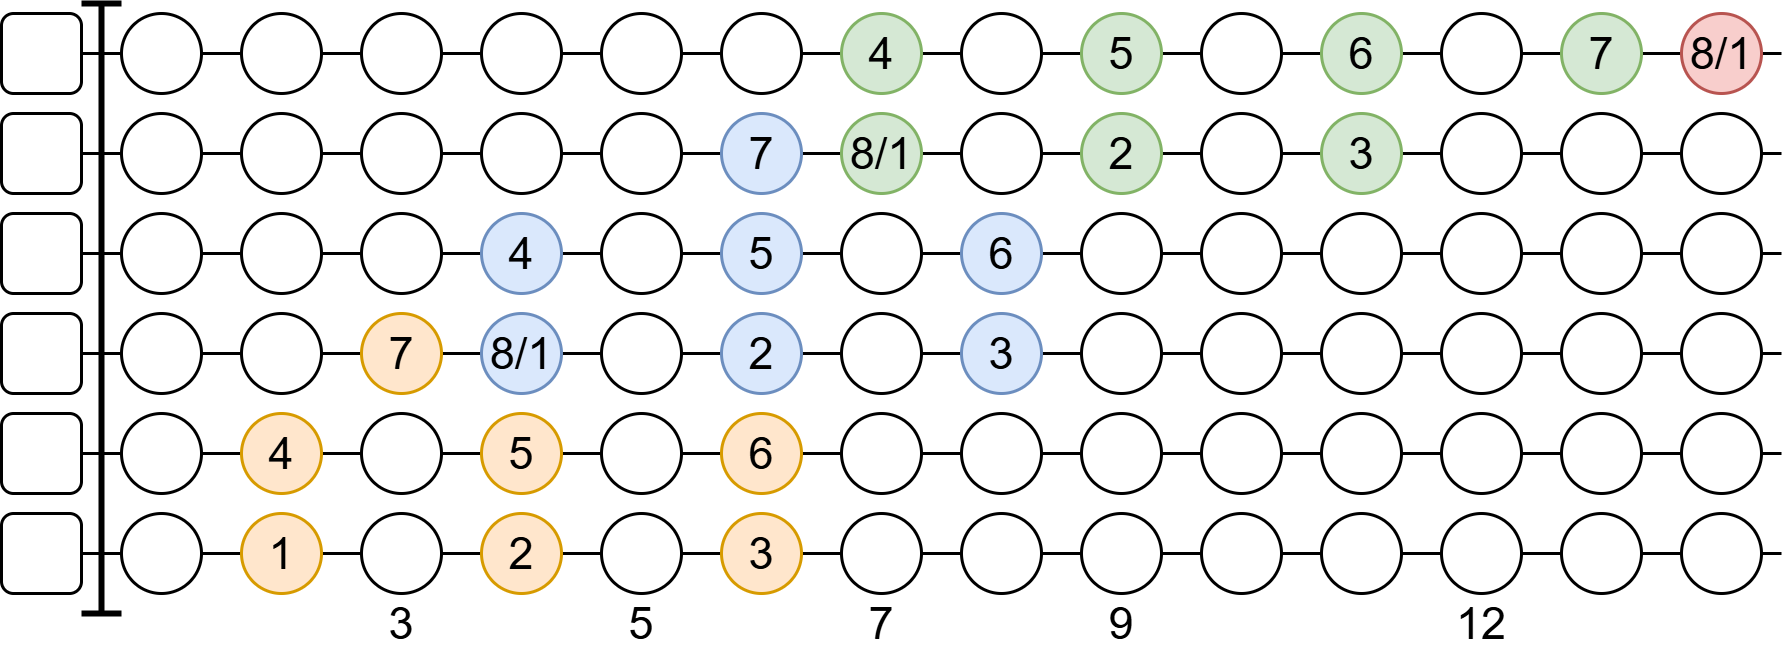
\includegraphics[height=0.18\textheight]{../../Images/guitar_major_scale_octaves_over_fretboard.png}
		\caption{Major scale octaves over the whole fretboard}
		\label{fig:guitar_major_scale_octaves_over_fretboard}
	\end{subfigure}
	
	\caption{F$\sharp$ major scale on the fretboard}
	\label{fig:guitar_major_scale_fretboard}
\end{figure}

\clearpage

The song "Tattoo" from "Loreen" uses the F$\sharp$ major scale. The main melody that you hear in the background is shown in \autoref{fig:guitar_tattoo_loreen_main_backing_melody}.

\begin{figure}[h]
	\centering
	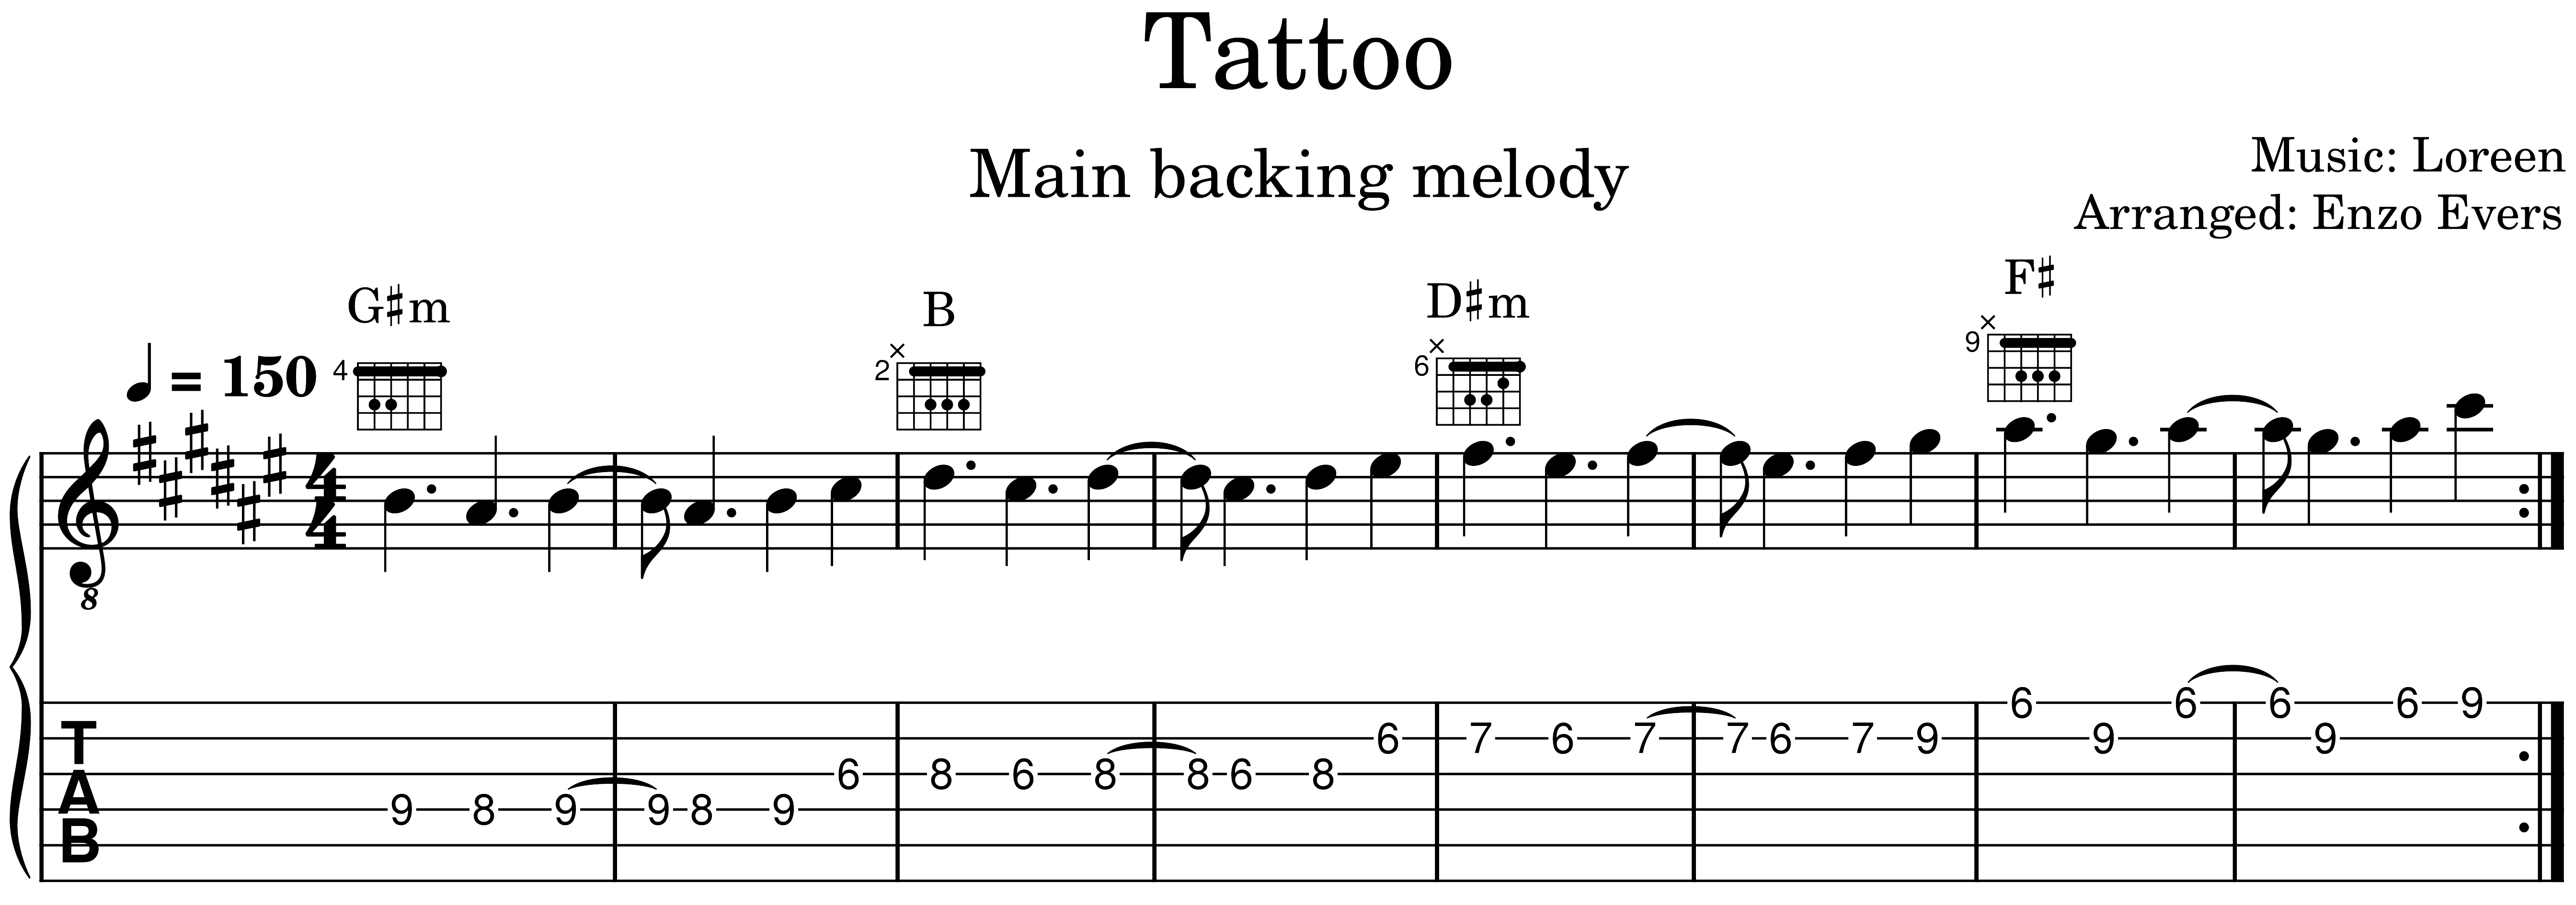
\includegraphics[width=\textwidth]{../../MuseScore/Guitar/LoreenTattooSimpleBackingMelody.png}
	\caption{Tattoo - Loreen main backing melody}
	\label{fig:guitar_tattoo_loreen_main_backing_melody}
\end{figure}

If you now compare the notes that are used, shown in \autoref{fig:guitar_tattoo_loreen_main_backing_melody_fretboard_major_scale}, and the multi-octave major scale of F$\sharp$ shown in \autoref{fig:guitar_major_scale_octaves_over_fretboard}, you will see that it nicely matches up.

The main differences are that the 'blue' 4 is now played on the 9th fret of the D string, and that the 'green' 3 is now played on the 6th fret of the high E string. Try to verify for yourself that these are indeed the same notes.

Because the number in the frets show the degree of the major scale we see that this melody covers all notes from the F$\sharp$ major scale (over show octaves). Note how all numbers 1 till 8 are used.

\begin{figure}[h]
	\centering
	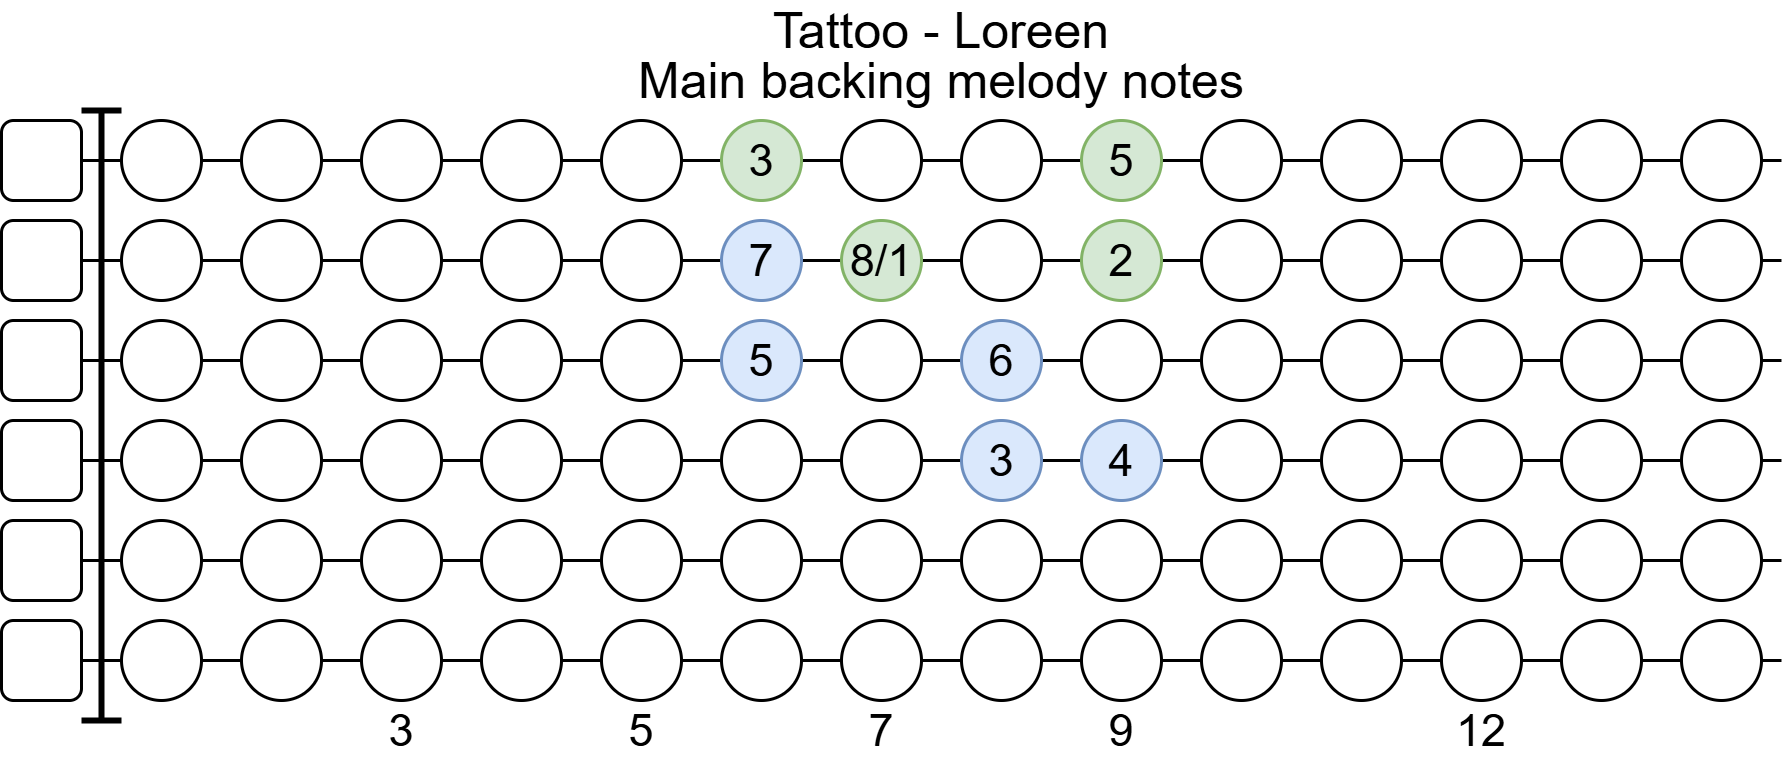
\includegraphics[height=0.2\textheight]{../../Images/NotesUsedInMainBackingMelodyTattooLoreen.png}
	\caption{Notes used in the main backing melody of "Tattoo - Loreen"}
	\label{fig:guitar_tattoo_loreen_main_backing_melody_fretboard_major_scale}
\end{figure}

\newpage

\subsection{The minor scale}

The minor diatonic scale has the formula shown in \autoref{tab:guitar_minor_scale_interval}.

\begin{table}[h]
	\centering
	\begin{tabular}{*{16}{c}}
		& \multicolumn{2}{P{4mm}}{\large{W}} & \multicolumn{2}{P{4mm}}{\large{H}} & \multicolumn{2}{P{4mm}}{\large{W}} & \multicolumn{2}{P{4mm}}{\large{W}} & \multicolumn{2}{P{4mm}}{\large{H}} & \multicolumn{2}{P{4mm}}{\large{W}} & \multicolumn{2}{P{4mm}}{\large{W}} & \\
		\multicolumn{2}{P{4mm}}{1} & \multicolumn{2}{P{4mm}}{2} & \multicolumn{2}{P{4mm}}{3$\flat$} & \multicolumn{2}{P{4mm}}{4} & \multicolumn{2}{P{4mm}}{5} & \multicolumn{2}{P{4mm}}{6$\flat$} & \multicolumn{2}{P{4mm}}{7$\flat$} & \multicolumn{2}{P{4mm}}{8}
	\end{tabular}
	\caption{Minor scale intervals}
	\label{tab:guitar_minor_scale_interval}
\end{table}

To create the A minor scale we will start on the A and then simply follow the formula.

\begin{table}[h]
	\centering
	\begin{tabular}{*{16}{c}}
		& \multicolumn{2}{P{4mm}}{\large{W}} & \multicolumn{2}{P{4mm}}{\large{H}} & \multicolumn{2}{P{4mm}}{\large{W}} & \multicolumn{2}{P{4mm}}{\large{W}} & \multicolumn{2}{P{4mm}}{\large{H}} & \multicolumn{2}{P{4mm}}{\large{W}} & \multicolumn{2}{P{4mm}}{\large{W}} & \\
		\multicolumn{2}{P{4mm}}{1} & \multicolumn{2}{P{4mm}}{2} & \multicolumn{2}{P{4mm}}{3$\flat$} & \multicolumn{2}{P{4mm}}{4} & \multicolumn{2}{P{4mm}}{5} & \multicolumn{2}{P{4mm}}{6$\flat$} & \multicolumn{2}{P{4mm}}{7$\flat$} & \multicolumn{2}{P{4mm}}{8} \\
		\multicolumn{2}{P{4mm}}{A} & \multicolumn{2}{P{4mm}}{B} & \multicolumn{2}{P{4mm}}{C} & \multicolumn{2}{P{4mm}}{D} & \multicolumn{2}{P{4mm}}{E} & \multicolumn{2}{P{4mm}}{F} & \multicolumn{2}{P{4mm}}{G} & \multicolumn{2}{P{4mm}}{A}
	\end{tabular}
	\caption{A minor scale}
	\label{tab:guitar_a_minor_scale}
\end{table}

Similar to example for the major scales of the natural notes, \autoref{tab:guitar_natural_note_minor_scale} shows the minor scales of the natural notes.

\begin{enumerate}
	\item \textbf{Each scale only has unique letters}. Therefore the 6th note in the D minor scale is a B$\flat$ and not an A$\sharp$.
	\item The 4th note in the scale is the start of the scale on the next row. Of course, this is because they are listed as such now. But it is the basis of the "circle of fourths" which we will learn more about later. Note that for the major scale this was the fifth note. Therefore the earlier mentioned "circle of fifth" applies to major scale, while the term "circle of fourths" applies to minor scale.
	\item Each scale below another in this list has one more $\flat$ than the previous. And the notes that have a flat in one scale, also have a flat in the scales below it. Again, this has to do with the "circle of fourths".
\end{enumerate}

\begin{table}[h]
	\centering
	\begin{tabular}{*{16}{c}}
		& \multicolumn{2}{P{4mm}}{\large{W}} & \multicolumn{2}{P{4mm}}{\large{H}} & \multicolumn{2}{P{4mm}}{\large{W}} & \multicolumn{2}{P{4mm}}{\large{W}} & \multicolumn{2}{P{4mm}}{\large{H}} & \multicolumn{2}{P{4mm}}{\large{W}} & \multicolumn{2}{P{4mm}}{\large{W}} & \\
		\multicolumn{2}{P{4mm}}{1} & \multicolumn{2}{P{4mm}}{2} & \multicolumn{2}{P{4mm}}{3$\flat$} & \multicolumn{2}{P{4mm}}{4} & \multicolumn{2}{P{4mm}}{5} & \multicolumn{2}{P{4mm}}{6$\flat$} & \multicolumn{2}{P{4mm}}{7$\flat$} & \multicolumn{2}{P{4mm}}{8} \\
		\multicolumn{2}{P{4mm}}{B} & \multicolumn{2}{P{4mm}}{C\sharp} & \multicolumn{2}{P{4mm}}{D} & \multicolumn{2}{P{4mm}}{E} & \multicolumn{2}{P{4mm}}{F\sharp} & \multicolumn{2}{P{4mm}}{G} & \multicolumn{2}{P{4mm}}{A} & \multicolumn{2}{P{4mm}}{B} \\
		\multicolumn{2}{P{4mm}}{E} & \multicolumn{2}{P{4mm}}{F\sharp} & \multicolumn{2}{P{4mm}}{G} & \multicolumn{2}{P{4mm}}{A} & \multicolumn{2}{P{4mm}}{B} & \multicolumn{2}{P{4mm}}{C} & \multicolumn{2}{P{4mm}}{D} & \multicolumn{2}{P{4mm}}{E} \\
		\multicolumn{2}{P{4mm}}{A} & \multicolumn{2}{P{4mm}}{B} & \multicolumn{2}{P{4mm}}{C} & \multicolumn{2}{P{4mm}}{D} & \multicolumn{2}{P{4mm}}{E} & \multicolumn{2}{P{4mm}}{F} & \multicolumn{2}{P{4mm}}{G} & \multicolumn{2}{P{4mm}}{A} \\
		\multicolumn{2}{P{4mm}}{D} & \multicolumn{2}{P{4mm}}{E} & \multicolumn{2}{P{4mm}}{F} & \multicolumn{2}{P{4mm}}{G} & \multicolumn{2}{P{4mm}}{A} & \multicolumn{2}{P{4mm}}{B\flat} & \multicolumn{2}{P{4mm}}{C} & \multicolumn{2}{P{4mm}}{D} \\
		\multicolumn{2}{P{4mm}}{G} & \multicolumn{2}{P{4mm}}{A} & \multicolumn{2}{P{4mm}}{B\flat} & \multicolumn{2}{P{4mm}}{C} & \multicolumn{2}{P{4mm}}{D} & \multicolumn{2}{P{4mm}}{E\flat} & \multicolumn{2}{P{4mm}}{F} & \multicolumn{2}{P{4mm}}{G} \\
		\multicolumn{2}{P{4mm}}{C} & \multicolumn{2}{P{4mm}}{D} & \multicolumn{2}{P{4mm}}{E\flat} & \multicolumn{2}{P{4mm}}{F} & \multicolumn{2}{P{4mm}}{G} & \multicolumn{2}{P{4mm}}{A\flat} & \multicolumn{2}{P{4mm}}{B\flat} & \multicolumn{2}{P{4mm}}{C} \\
		\multicolumn{2}{P{4mm}}{F} & \multicolumn{2}{P{4mm}}{G} & \multicolumn{2}{P{4mm}}{A\flat} & \multicolumn{2}{P{4mm}}{B\flat} & \multicolumn{2}{P{4mm}}{C} & \multicolumn{2}{P{4mm}}{D\flat} & \multicolumn{2}{P{4mm}}{E\flat} & \multicolumn{2}{P{4mm}}{F}
	\end{tabular}
	\caption{Minor scales of all natural notes}
	\label{tab:guitar_natural_note_minor_scale}
\end{table}

\newpage

Just as for the major scale, there are different patterns for the minor scale (\autoref{fig:guitar_minor_scale_fretboard}). The numbers correspond to the interval in the scale. The scale that you are playing is determined by the root note (the "1" note). In this example we are therefore playing the F$\sharp$ minor scale. If you would move all notes up by 1 fret, you would be playing the G minor scale.

The different colors in \autoref{fig:guitar_minor_scale_fretboard_standard} indicate different octaves. This is the 'standard'/compact minor scale shape. Note how the frets with "8/1" indicate the 8 of the previous octave, and the 1 of the next octave.

Learning these shapes by heart makes it easy to improvise over a song. But more important is to see how these shapes relate to the intervals of the minor scale. The easiest shape for this is \autoref{fig:guitar_minor_scale_fretboard_single_string}. With this shape you can easily recognize the minor diatonic scale formula (w-h-w-w-h-w-w). All shapes have the same notes, just played on a different position on the fretboard and possibly in a different octave. The shapes shown below don't cover all possibilities yet.

The F$\sharp$ minor scale has the following notes:

\begin{table}[h]
	\centering
	\begin{tabular}{*{16}{c}}
		& \multicolumn{2}{P{4mm}}{\large{W}} & \multicolumn{2}{P{4mm}}{\large{H}} & \multicolumn{2}{P{4mm}}{\large{W}} & \multicolumn{2}{P{4mm}}{\large{W}} & \multicolumn{2}{P{4mm}}{\large{H}} & \multicolumn{2}{P{4mm}}{\large{W}} & \multicolumn{2}{P{4mm}}{\large{W}} & \\
		\multicolumn{2}{P{4mm}}{1} & \multicolumn{2}{P{4mm}}{2} & \multicolumn{2}{P{4mm}}{3$\flat$} & \multicolumn{2}{P{4mm}}{4} & \multicolumn{2}{P{4mm}}{5} & \multicolumn{2}{P{4mm}}{6$\flat$} & \multicolumn{2}{P{4mm}}{7$\flat$} & \multicolumn{2}{P{4mm}}{8} \\
		\multicolumn{2}{P{4mm}}{F$\sharp$} & \multicolumn{2}{P{4mm}}{G$\sharp$} & \multicolumn{2}{P{4mm}}{A} & \multicolumn{2}{P{4mm}}{B} & \multicolumn{2}{P{4mm}}{C$\sharp$} & \multicolumn{2}{P{4mm}}{D} & \multicolumn{2}{P{4mm}}{E} & \multicolumn{2}{P{4mm}}{F$\sharp$}
	\end{tabular}
	\caption{F$\sharp$ minor scale}
	\label{tab:guitar_f_sharp_minor_scale}
\end{table}

\autoref{fig:guitar_f_sharp_minor_scale_score_multi_octave} shows the notes that correspond to \autoref{fig:guitar_minor_scale_octaves_over_fretboard}.

\begin{figure}[h]
	\centering
	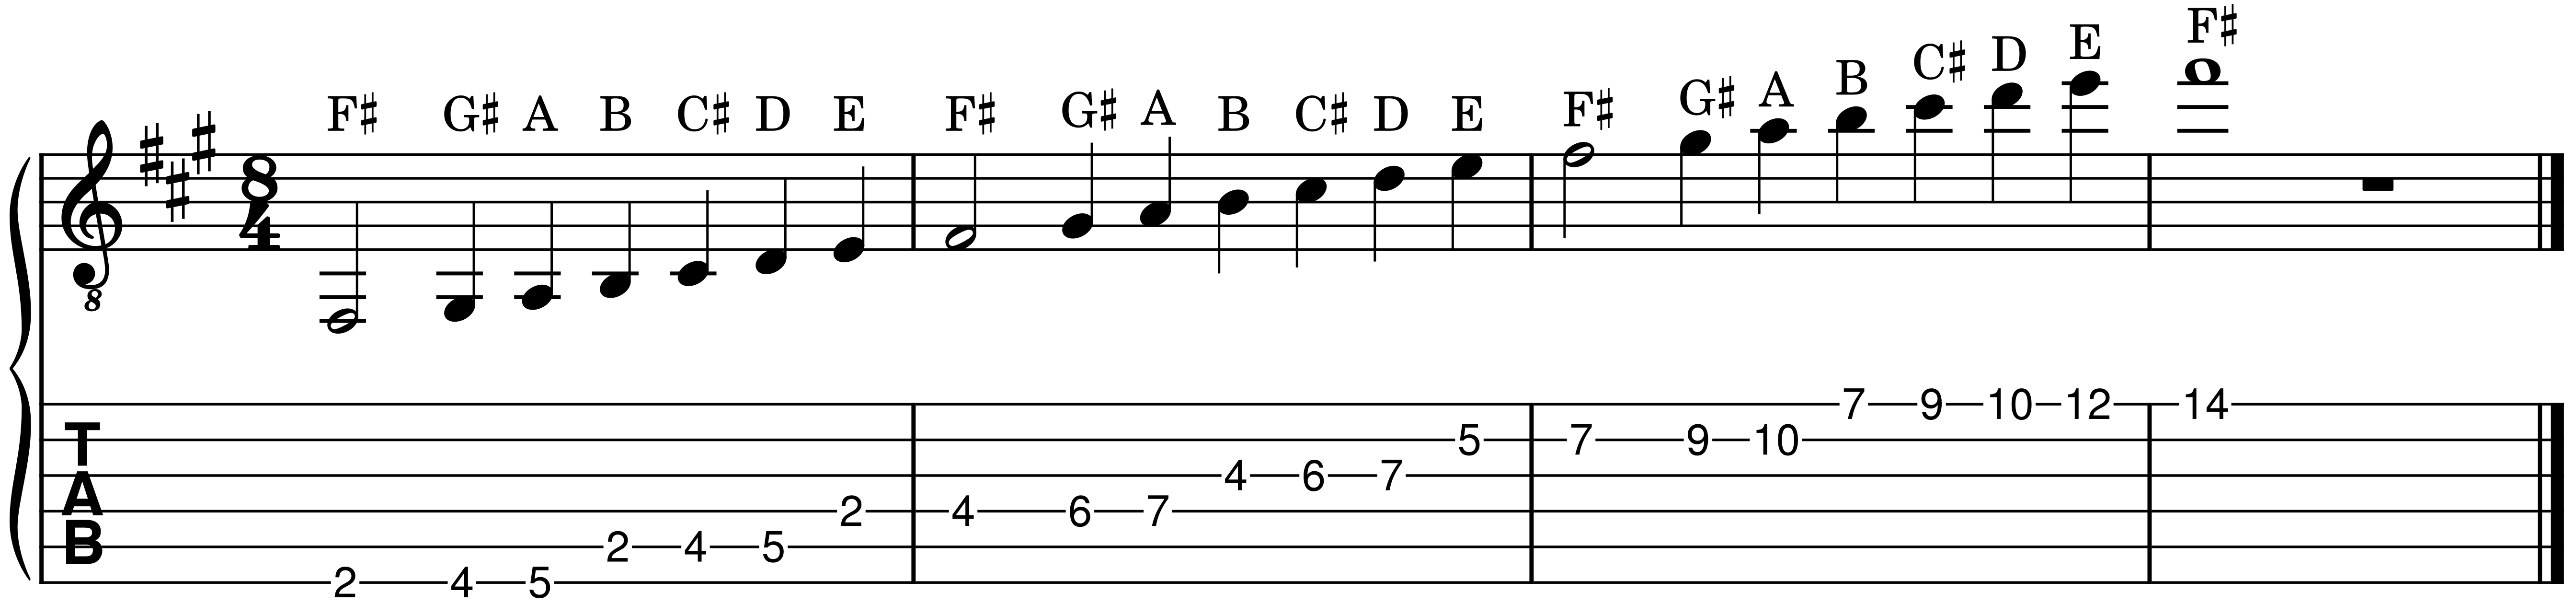
\includegraphics[width=\textwidth]{../../MuseScore/Guitar/GuitarFSharpMinorMultiOctave.png}
	\caption{Multiple octaves of the F$\sharp$ minor scale}
	\label{fig:guitar_f_sharp_minor_scale_score_multi_octave}
\end{figure}

\newpage

\begin{figure}[h]
	\begin{subfigure}[b]{0.45\textwidth}
		\centering
		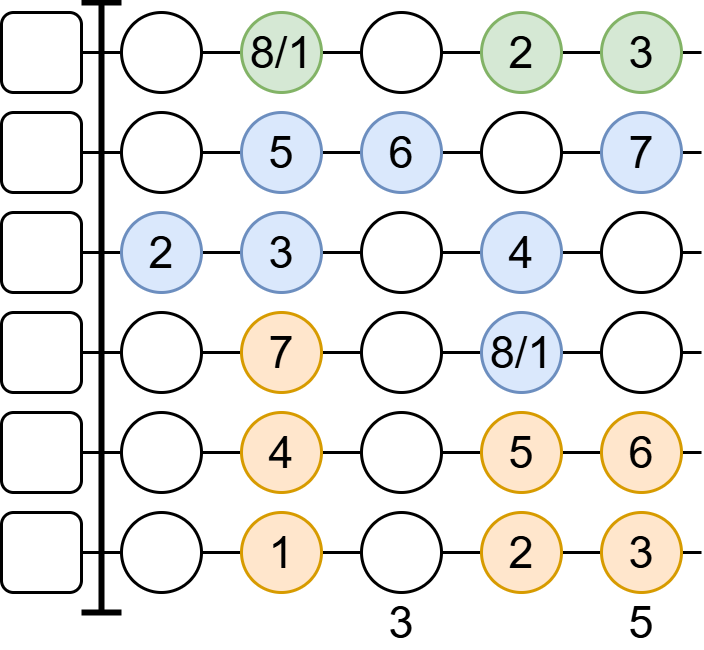
\includegraphics[height=0.175\textheight]{../../Images/guitar_minor_scale_standard.png}
		\caption{Minor scale on the fretboard (standard)}
		\label{fig:guitar_minor_scale_fretboard_standard}
	\end{subfigure}
	\hfill
	
	\vspace{0.5cm}
	\begin{subfigure}[b]{\textwidth}
		\centering
		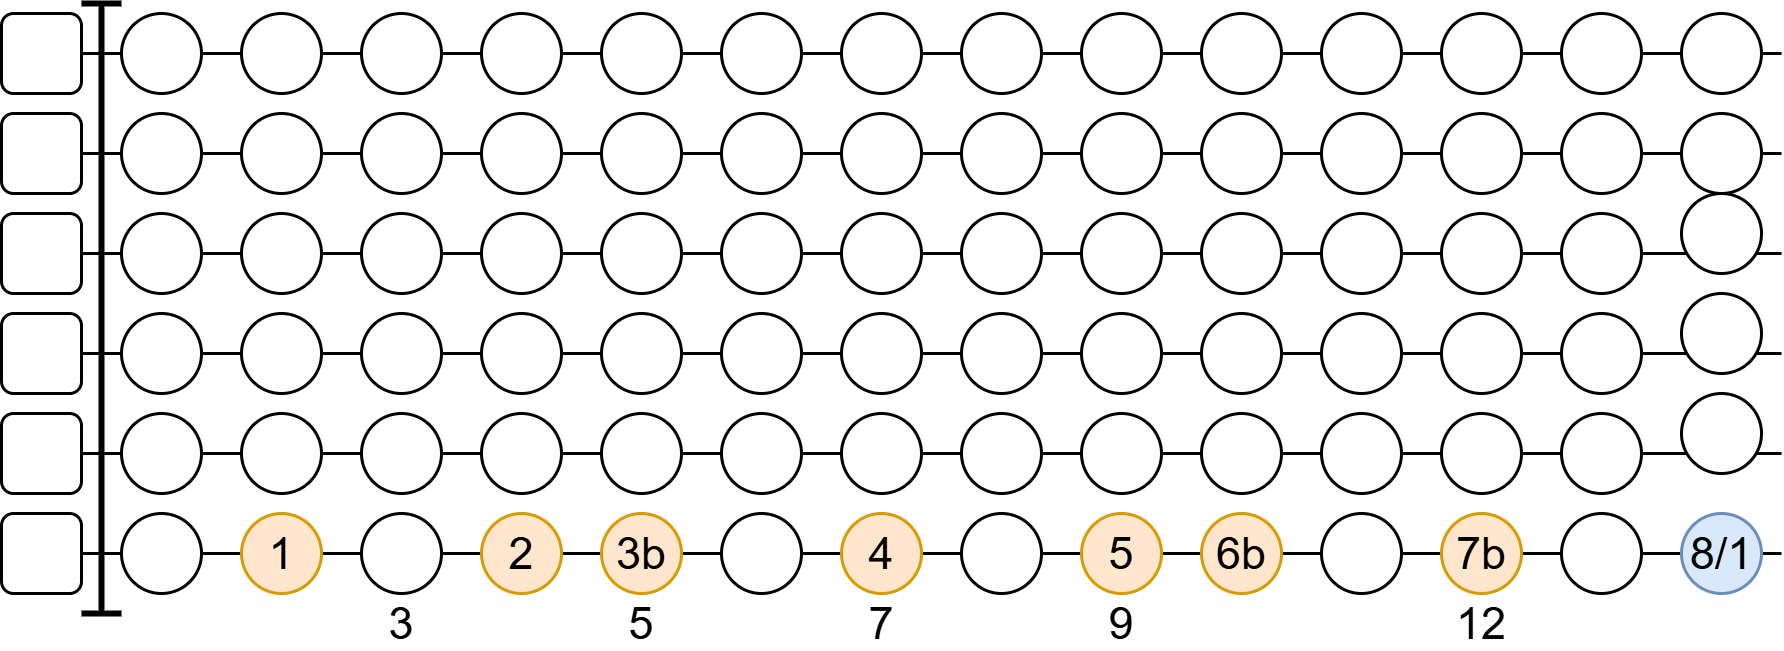
\includegraphics[height=0.175\textheight]{../../Images/guitar_minor_scale_single_string.png}
		\caption{Minor scale on the fretboard on a single string}
		\label{fig:guitar_minor_scale_fretboard_single_string}
	\end{subfigure}
	
	\vspace{0.5cm}
	\begin{subfigure}[b]{\textwidth}
		\centering
		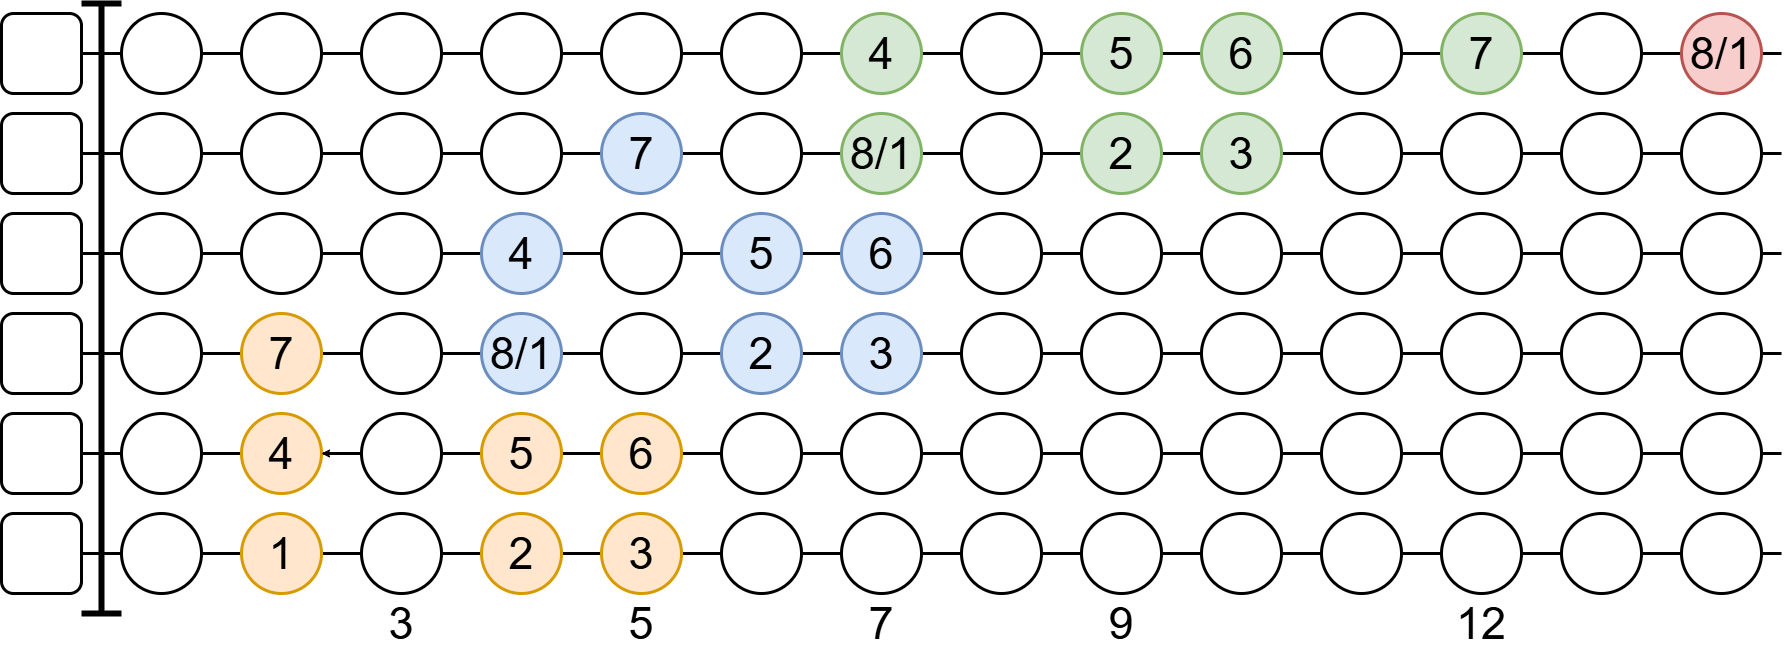
\includegraphics[height=0.175\textheight]{../../Images/guitar_minor_scale_octaves_over_fretboard.png}
		\caption{Minor scale octaves over the whole fretboard}
		\label{fig:guitar_minor_scale_octaves_over_fretboard}
	\end{subfigure}
	
	\caption{F$\sharp$ minor scale on the fretboard}
	\label{fig:guitar_minor_scale_fretboard}
\end{figure}

\clearpage

The song "The Final Countdown" from "Europe" is in F$\sharp$ minor. The intro is shown in \autoref{fig:guitar_the_final_countdown_europe_intro}.

\begin{figure}[h]
	\centering
	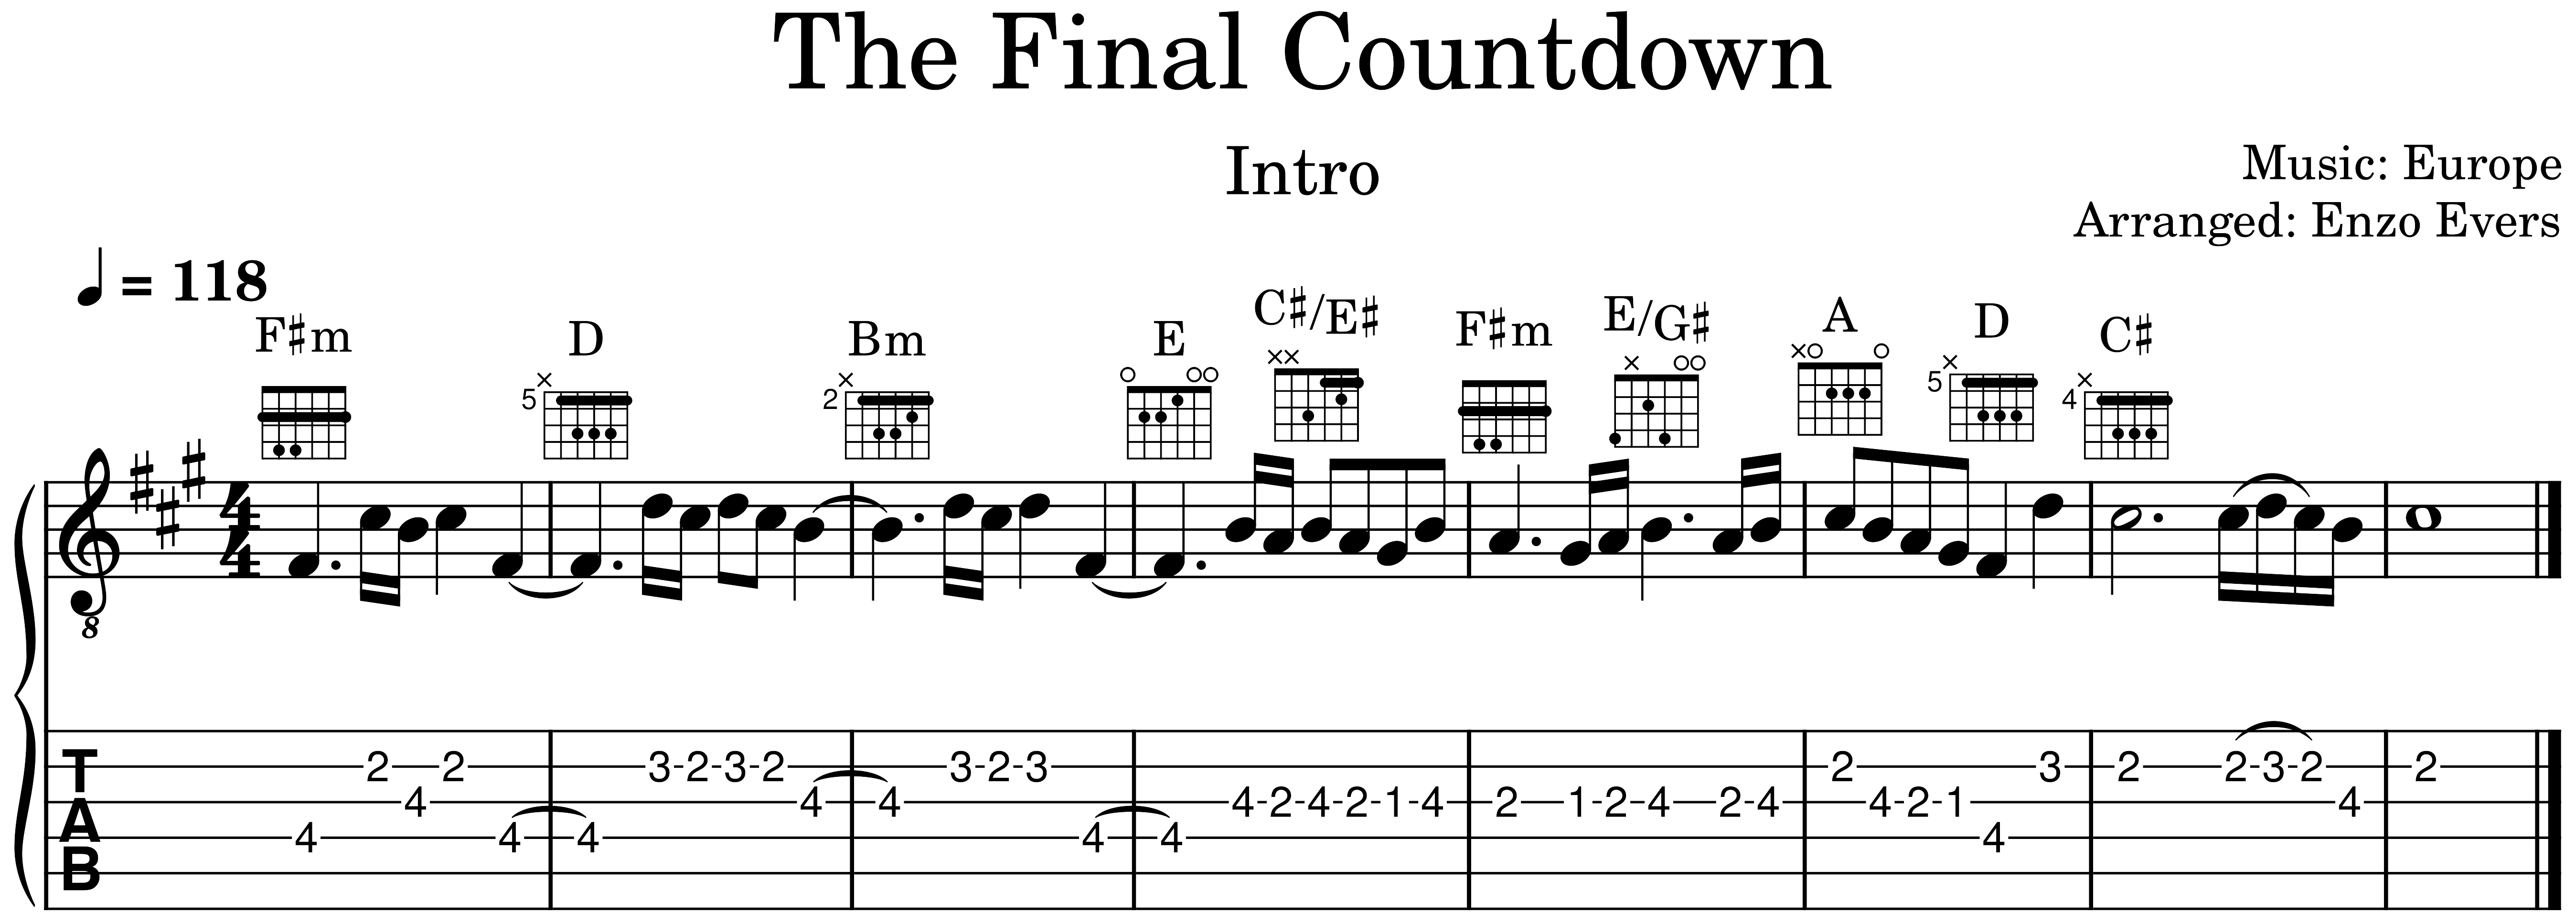
\includegraphics[width=\textwidth]{../../MuseScore/Guitar/GuitarTheFinalCountdownEuropeIntro.png}
	\caption{The Final Countdown - Europe intro}
	\label{fig:guitar_the_final_countdown_europe_intro}
\end{figure}

Looking at the notes used, you see that it nicely overlaps with the F$\sharp$ minor scale shown in \autoref{fig:guitar_minor_scale_fretboard_standard}. Just as in the previous fretboard diagrams, the numbers in the circles indicate the degree in the, in this case minor, scale.

\begin{figure}[h]
	\centering
	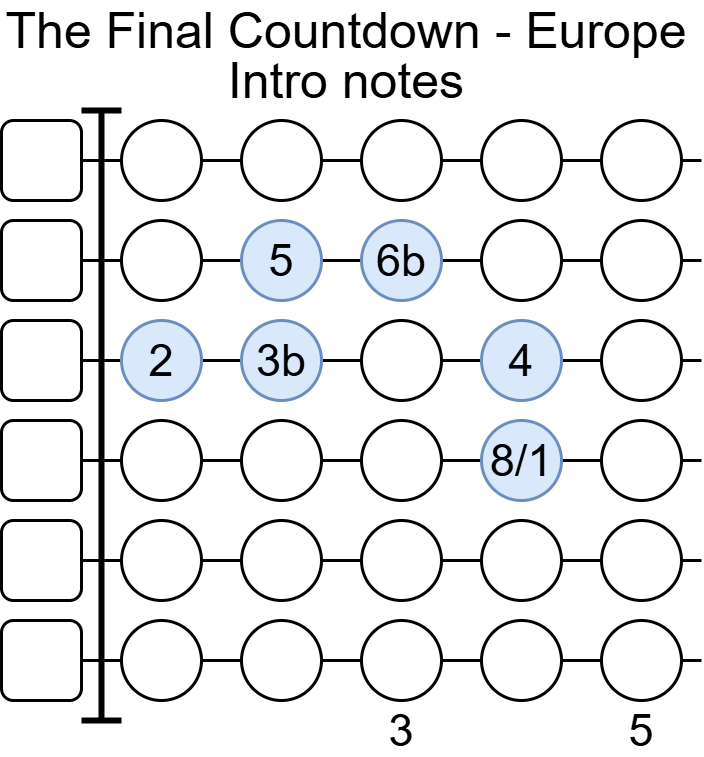
\includegraphics[height=0.2\textheight]{../../Images/NotesUsedInTheFinalCountdownEuropeIntro.png}
	\caption{Notes used in the intro of "The Final Countdown - Europe"}
	\label{fig:guitar_the_final_countdown_europe_fretboard_minor_scale}
\end{figure}


% I don't particularly like modes a lot.